\chapter{Datasets used}
To give an overview of the data used as well as extend the scheme presented in
the Introduction chapter (Figure~\ref*{fig:workflow}), refer to Figure~\ref*{fig:data_flow}.
The following sections provide more details about the data.

\begin{figure}[h]
  \centering
  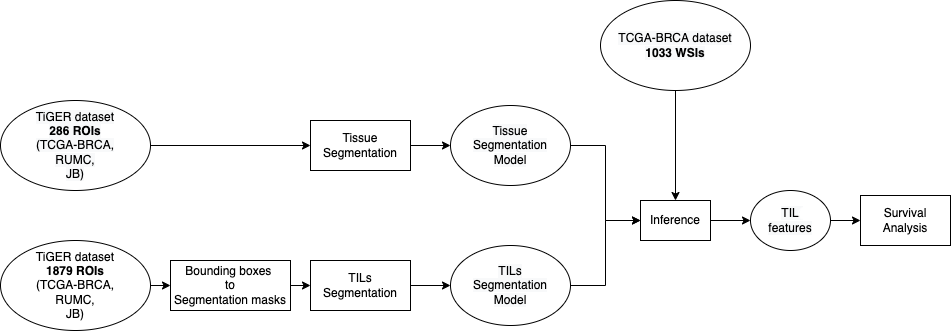
\includegraphics[width=\linewidth]{figures/data_flow.png} 
  \caption{Workflow in form of a Petri net showing completed tasks in this thesis complemented with the data sources and counts.
  For training, validation, and testing of segmentation models only TiGER challenge data was used, originating from three medical institutes (TCGA-BRCA, RUMC, and JB).
  Calculation of TIL features was performed on TCGA-BRCA diagnostic slides.} 
  \label{fig:data_flow}
\end{figure} 

\section{Segmentation} \label{section:data_segmentation}
The data for tissue and TILs segmentation originates from publicly available
Tumor InfiltratinG lymphocytes in breast cancER (TiGER) challenge dataset containing
digital pathology images of Her2 positive (Her2+) and Triple Negative (TNBC) breast
cancer whole-slide images (WSIs), regions of interest (ROIs), and manual annotations.
More specifically, the WSIROIS dataset was used for model training, validation, and
testing (see Table~\ref*{tab:segm_data}).
It includes 195 WSIs of breast cancer core-needle biopsies and surgical resections with
pre-selected ROIs and manual annotations.
TiGER data, both at WSI and ROI level, was released at a spacing (pixel size) of
approximately 0.5 \textmu m/px (at 20$\times$ magnification ), more information is available on the original
challenge website\footnote{\url{https://tiger.grand-challenge.org/Data/}}.
\begin{table}[h!]
\centering
\begin{tabular}{ l c c c c c c } 
\hline
\multirow{3}{*}{Source} &  \multicolumn{3}{c}{Tissue} & \multicolumn{3}{c}{TILs}\\ 
\cline{2-7}
 & slides & ROIs & median ROI size & slides & ROIs & median ROI size \\ 
  & & & \#pixels [k] & & & \#pixels [k] \\ 
\hline
TCGA-BRCA & 151 & 151 & 4 983 & 124 & 1744 & 20\\ 
RUMC & 26 & 81 & 1 312 & 26 & 81 & 1 312\\ 
JB & 18 & 54 & 1 465 & 18 & 54 & 1 465\\
\hline
 & 195 & 286 & & 168 & 1879 &\\
\end{tabular}
\caption{\label{tab:segm_data}TiGER data overview. Sources: Cancer Genome Atlas Breast Invasive Carcinoma (TCGA-BRCA),
Radboud University Medical Center (RUMC) and Jules Bordet Institute (JB). Tissue slides and ROIs refer to the segmentation
images and annotations whereas TILs prefix specifies the data for TILs detection provided by the challenge.
TCGA-BRCA dataset statistics showcase a variation in ROIs sizes for tissue and TILs tasks as well as compared to two other datasets.}
\end{table}
The TiGER tissue annotations include eight
labels that were reduced to three (see Table~\ref*{tab:label_data}).
The training masks were generated using available XML files.
Within provided mask images, in certain cases, regions not included in ROIs and non-annotated regions were marked with the same label, which could not be directly used for training (see ground truth in Figure~\ref*{fig:TCGA-GM-A2DF}).
\begin{table}[h!]
\centering
\begin{tabular}{ l c c c c } 
\hline
TiGER Tissue Label & Share & ID & new ID & new Tissue Label \\ 
\hline
Invasive tumor & 0.283 & 1 & 1 & Tumor\\ 
In-situ tumor & 0.029 & 3 & 1 & Tumor\\ 
Tumor-associated stroma & 0.286 & 2 & 2 & Stroma\\
Inflamed stroma & 0.096 & 6 & 2 & Stroma\\
Necrosis not in-situ & 0.048 & 5 & 0 & Rest\\
Healthy glands & 0.0008 & 4 & 0 & Rest\\ 
Background & 0.231 & 0 & 0 & Rest\\ 
Rest & 0.026 & 7 & 0 & Rest\\
\hline
\end{tabular}
\caption{\label{tab:label_data} Reduction of labels provided in TiGER challenge dataset. Resulting labels include three classes: Tumor (1), Stroma (2) and Rest (0) with shares of 0.312, 0.382 and 0.306. Shares were calculated by dividing
the number of pixels belonging to some label by the number of the pixel in the current image and averaged over all images. }
\end{table}
While for tissue segmentation the images and their masks could be used directly as extracted from the dataset, the data for TILs segmentation required some preprocessing.
The TiGER fixed-size bounding box annotation for lymphocytes and plasma cells (see Table~\ref{tab:tils_data}) was adapted for segmentation by transforming each bounding box into an annotation of the center pixel with a dilatation of three.
\begin{table}[h!]
\centering
\begin{tabular}{ l c c c c c c } 
\hline
\multirow{2}{*}{Source} & & & & \multicolumn{3}{c}{Number of cells per ROI}\\ 
\cline{2-7}
 & slides & ROIs & cells & min & max & median \\ 
\hline
TCGA-BRCA & 124 & 1 744 & 19 115 & 0 (44.3\%) & 206 & 1\\ 
RUMC & 26 & 81 & 4 728 & 0 (7.4\%) & 657 & 19\\ 
JB & 18 & 54 & 5 523 & 0 (7.4\%) & 608 & 51.5\\
\hline
 & 168 & 1 879 & 29 366 & & &\\
\end{tabular}
\caption{\label{tab:tils_data} Data overview for TILs detection. Sources: Cancer Genome Atlas Breast Invasive Carcinoma (TCGA-BRCA),
Radboud University Medical Center (RUMC) and Jules Bordet Institute (JB). Number of cells here refers to the number of
bounding boxes that were assigned for lymphocytes and plasma cells, further named TILs.
Increased number of ROIs compared to tissue segmentation task, only due to TCGA-BRCA dataset and its considerably smaller ROIs as summarized in Table~\ref{tab:segm_data}.}
\end{table}

For the inferences the breast cancer TCGA-BRCA dataset was used, generated by
the TCGA Research Network: \hyperlink{https://www.cancer.gov/tcga}{https://www.cancer.gov/tcga}.
While there are a large number of images available in The Cancer Genome Atlas (TCGA),
only the diagnostic slide were downloaded (Formalin-Fixed Paraffin-Embedded (FFPE) slides).
FFPE slides are the gold standard in diagnostic medicine~\cite{smith_2014}.
They are prepared by fixing a specimen in formaldehyde and then placing it in a
paraffin block to section it. 
After generating a manifest file on TCGA dataset website, which includes 1133 diagnostic slides
of BRCA breast cancer patients, the files were downloaded with the GDC Data Transfer Tool
(\verb+gdc-client+ with \verb+--manifest+ option). 


\section{Survival Analysis}
The TiGER challenge aims to assess the prognostic significance of computer-generated TILs scores for predicting survival by applying the Cox proportional hazards model. The survival analysis was done using a large independent dataset that includes cases from both clinical routine and from a phase 3 clinical trial.
200 WSIs and their clinicopathological variables, including recurrence and survival data were used as the experimental set, and 707 cases for the test set, both not directly accessible to participants.

The survival analysis within this thesis is done exclusively on publicly available TCGA-BRCA data.
The first twelve characters of the TCGA barcode identifiers are saved under \texttt{case\_submitter\_id}
as a unique patient identifier. 
In the dataset, death (\texttt{vital\_status} = 1) is considered as an event, and the time until the
event or censoring is either \texttt{days\_to\_death} (number of days to death from the first diagnosis)
or \texttt{days\_to\_followup} (number of days to last follow-up from the first diagnosis). The patients
that had missing values, that are essential for survival analysis (\texttt{case\_submitter\_id},
\texttt{vital\_status} and time to event) were filtered out. The resulting dataset includes clinical
variables for 1076 patients with 150 events.
Originally the time is recorded in days, but it was converted to years (by simply dividing by 365),
due to the fact that the mean duration until censoring is 3.3 years and 4.4 years until death,
and the maximum duration until censoring reaches 23.6 years and 20.4 years until death. 
The final number of patients that are included in the survival analysis and have corresponding diagnostic slide(s) is 1015.

Additionally, a further file (nationwidechildrens.org\_clinical\_patient\_brca.txt)
was downloaded from the TCGA portal. It includes Her2, estrogen, and progesterone
receptor levels measured in a primary tumor or metastases with immunohistochemistry.
115 TNBC and 159 Her2+ patients were identified, by filtering columns
\texttt{er\_status\_by\_ihc}, \texttt{pr\_status\_by\_ihc} and \texttt{her2\_status\_by\_ihc}.
This dataset also includes the earlier mentioned columns that are essential for survival analysis, but the durations and
vital statuses are not kept up-to-date, thus the previous survival data was used with extracted patient identifiers
depending on the receptor levels.
